\documentclass[11pt]{article}
\usepackage{setspace}
\setstretch{1}
\usepackage{amsmath,amssymb, amsthm}
\usepackage{graphicx}
\usepackage{bm}
\usepackage[hang, flushmargin]{footmisc}
\usepackage[colorlinks=true]{hyperref}
\usepackage[nameinlink]{cleveref}
\usepackage{footnotebackref}
\usepackage{url}
\usepackage{listings}
\usepackage[most]{tcolorbox}
\usepackage{inconsolata}
\usepackage[papersize={8.5in,11in}, margin=1in]{geometry}
\usepackage{float}
\usepackage{caption}
\usepackage{esint}
\usepackage{url}
\usepackage{enumitem}
\usepackage{subfig}
\usepackage{wasysym}
\newcommand{\ilc}{\texttt}
\usepackage{etoolbox}
\usepackage{algorithm}
\usepackage{changepage}
% \usepackage{algorithmic}
\usepackage[noend]{algpseudocode}
\usepackage{tikz}
\usetikzlibrary{matrix,positioning,arrows.meta,arrows}
\patchcmd{\thebibliography}{\section*{\refname}}{}{}{}
% \PassOptionsToPackage{hyphens}{url}\usepackage{hyperref}

\providecommand{\myceil}[1]{\left \lceil #1 \right \rceil }
\providecommand{\myfloor}[1]{\left \lfloor #1 \right \rfloor }


\begin{document}



\title{\textbf{CSDS 455: Take Home Final}}

\author{Shaochen (Henry) ZHONG, \ilc{sxz517}}
\date{Started around 11:50, submitted before 15:00 12/10/2020 \\ Fall 2020, Dr. Connamacher}
\maketitle



\section*{Problem 1}

If $G \cong H$, then for every $e_G \in E(G)$ there must be a corresponding $e_H \in E(H)$, and for every $v_G \in V(G)$ there must be a corresponding $v_H \in V(H)$. Which suggests there is a bijection of $f: V(G) \rightarrow V(H)$. This imples if we have an $xy \not \in E(G)$, we will also have $f(x)f(y) \not \in E(H)$ for $x, y \in V(G), V(H)$.

Then we know such $xy$ must be $\in E(\overline{G})$ by the definition of complement. This means for every edge $e$ that is not in $G$, it must be also not in $H$, but in $\overline{G}$ and in $\overline{H}$. Thus we may have an one-to-one relationship for edges in $\overline{G}$ to edges in $\overline{H}$, and combined with the fact that $G, H, \overline{G}, \overline{H}$ all have the same vertex set, this implies $\overline{G} \cong \overline{H}$.\newline

The other direction is trivial to show as $\overline{\overline{G}} = G$. We may simply set two isomorphic graphs $G_1, H_1$ to be denoted as $\overline{G_2}, \overline{H_2}$; and as we know there must be $\overline{G_1} \cong \overline{H_1}$ by the pervious proof, there must also be $G_2 \cong H_2$ as they are the complments of $\overline{G_2}, \overline{H_2}$.

\section*{Problem 2}

WLOG, assume we are dealing with $k$-regular bipartite graph $G$. Known that every $v \in V(G)$, we have $d(v) = k$, we may therefore partition $G$ into set $U, V$ where $|U| = |V|$ -- this is true because due to the bipartite nature, every edge from a vertex in $U$ goes to a vertex in $V$, the total number of edges from $U \rightarrow V$  is the same as $V \rightarrow U$.

Assume we have $S \subseteq U$. We denotes edges connect to $S$ and $N(S)$ to be $E(S)$ and $E(N(S))$. Known that $|E(S)| = k|S|$ due to the nature of being $k$-regular, we have $k|S|$ number of edges from $S \rightarrow V$. On the other hand, we must have $k|N(S)|$ number of edges from $N(S) \rightarrow U$. Known $E(N(S))$ may include edges from $U - S$, we must have $k|N(S)| \geq k|S|$, which suggests $|S| \leq |N(S)|$.\newline

Thus, the \textsc{Hall's} condition is achieved and we may have a matching $M$ where $|E(M)| = |U|$, and known that $|U| = |V|$, this matching will include all verticies of $G$ and thus a perferct matching of $G$.


\section*{Problem 3}

For a $k$-connected graph $G$, we know the minimum vertex cut of $G$ is of size $k$; and by \textsc{Menger's} theorem we know that there must be $k$ vertex-disjoint-path from $u \to v$ for any $u, v \in V(G)$. If by contracting edge $xy$ will result in $G'$ ($G$ with $xy$ contracted) being no longer $k$-connected, this suggests $G'$ must has less than $k$ vertex-disjoint-path; which is only possible if $x$ and $y$ are on two different vertex-disjoint-path of $G$, therefore by contracting them together we have merged two disjoint pathes into one and made $G'$ no longer $k$-connected.

This also suggests for $e = xy$, $e$ is not part of any of the $k$ vertex-disjoint-path in $G$, thus $G-e$ will not affect the connectivity of graph and therefore still $k$-connected.


\section*{Problem 4}

By having the $a \to b$ path having at least two vertices on the $k$ vertex-disjoint-path of $u_i \to v_i$ it ``touches,'' we may skip the gap between the two vertices on of $a \to b$ on every vertex disjoint path, use the two end, and have one extra vertex-disjoint-path between $\{a, b, u_1, ..., u_k, v_1, ..., v_k\}.$ The new set of vertex-disjoint-path are depicted by the blue lines in the below graph:

\begin{figure}[H]
    \centering
    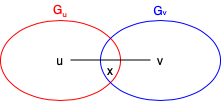
\includegraphics[width= 0.8\linewidth]{{fig/fig_p4_1.png}}
\end{figure}

So if we have $u_1 \to v_1, u_2 \to v_1, ..., u_k \to v_k$, we may have $k+1$ vertex-disjoint-pathes being $a \to x_1 \to u_1, v_1 \to y_1 \to u_2,  v_2 \to y_2 \to u_3, ..., v_k \to y_3 \to b$.

\section*{Problem 5}
I love graph theory :(

\section*{Problem 6}

For the question Since $G$ is color-critical, assuming $G$ has a bridge $xy$, removing the edge $xy$ will result in $G-xy$ being $\Delta(G)$ colorable. As $xy$ is a bridge, $G-xy$ will have two components $G_x$ and $G_y$, and and both of them must be $\Delta(G)$ colorable. This suggests $x, y$ should have at most $\Delta(G) - 1$ degree (as the graph $G$ may at most have $\Delta(G)$ by definition, not with $xy$ removed from $x$ and $y$, their maximum possible degree decrease by one).

Also known that $G_x$ and $G_y$ are two independent components, we may legally recolor the edges connecting to $y$ to be using the same $\Delta(G) - 1$ colors of edges connecting to $x$ (WLOG, we can also recolor $x$ as $y$). And then we can use the $\Delta(G)$-th color to color the $xy$ bridge and thus color $G$ with only $\Delta(G)$ colors -- which is a contradition to the problem's setup and $G$ is therefore bridgeless.

\noindent (for this question ``colorable'' means ``edge-colorable'')

\section*{Problem 7}

Known that $G$ has a nowhere-zero 2-flow, which means for every edage in $G$ we have a flow of $-1$ or $1$, and we can make every edge monotonically flow $1$ by flipping the direction of edge with flow $-1$.

As every edge has flow $1$, if we have $k$ edges going into vertex $x \in V(G)$, there must also be $k$ edges out of $x$. WLOG, assume we have edge $xy$ being $x \to y$ and now we removed this edge $xy$ from $G$. As $G-xy$ will still be bridgeless, we know that $d(x) \geq 4$ in $G$ because we know that $d(x) \neq 1, 3$ due to it must have the same amount of in-flow to out-flow edges, and there must also be $d(x) \neq 2$ as otherwise with $xy$ removed, $G-xy$ is no longer bridgeless (the edge connects to $x$ is a bridge).

So $x$ will still have at least $2$-flow as ``in-edges,'' but now with one less ``out-edge,'' there must be another out-edge from $x$ to have a flow value of $2$ to balance the input-output circulation. And this $2$-flow out-edge from $x$, say it is $x \to v$ (WLOG) will make another out edge from $v$ to carry a $2$-flow... eventually, the abosulte flow value of the graph $G-xy$ will be $1, 2$, which means $G-xy$ now has a nowhere-zero 3-flow.

\section*{Problem 8}

For any graph $G$, given a tree decomposition $T(G)$ where $tw(T(G)) \leq k$ -- as among all the possible tree decompositions of $G$, the one tree decomposition with minimum treewidth can be the $T(G)$. As we are trying to show having treewidth at most $k$ is a hereditary property, we consider edge deletion, vertex deletion, and edge contraction seperatly.

\begin{itemize}
    \item Assume we obtain $G'$ from $G$ by conducting an edge delection of $uv$. The $T(G')$ can be same as $T(G)$ as the only requirment regarding edge $e$ in $G$ to $T(G)$ is to have two ends of $e$ in the at least one bag of $T(G)$, and removing $e$ does not require further modification of $T(G)$.
    \item Assume we obtain $G'$ from $G$ by conducting a vertex delection of $u$. We may simply remove all apperance of $u$ in the bags of $T(G)$ and this can be our $T(G')$.
    \item Assume we obtain $G'$ from $G$ by conducting an edge contraction of $uv$ to $w$, we may simply replace all apperance of $u$ or $v$ as $w$ in $T(G)$ to be our $T(G')$. This replacement is legal as for every edge with one end to $u$ and $v$ in $G$, such egde will now be connected to $w$ in $G'$, and having $w$ as replacement of $u, w$ will maintain the ``for every edge in $G$ such edge must have its two ends in at least one bag of $T$'' property. So $T(G')$ will have the same structure of $T(G)$.
\end{itemize}

As every $T(G')$ in all scenarios will share the same tree structure of $T(G)$, and for all scenarios we never increase of vertex in bags of $T(G)$, we must have $tw(T(G')) \leq k$ given $tw(T(G)) \leq k$. By induction, we may say that for all minor $H$ of $G$,  $tw(T(H)) \leq k$ given that $tw(T(G)) \leq k$.

\section*{Problem 9}

We know that we may find all vertex seperation set of $k+1$ size in polynomial time of $O(n^{k+1})$, so we first find the useable tree decomposisions of $G$. Then the general idea is to do a bottom up traversal from the leaf to the root of the tree.

We try to identify, depending on the given question, that if there is a subproblem we can work ON within the currect leaf bag. We register some necessary boolean valueS in a table, then we proceed to do the same with it's parent bag.\newline

Take \textsc{Hamiltonian} cycle as an example, we first identify all the possible extrance/exit pairs within a bag -- which is an combinatory expression that at most goes to power of $O(k+1)$ . Then we register if a vertex is on a Hamiltonian cycle within the current bag, or if such vertex will be convered in the parent bag's HC. We will usually register this kind of information as boolean values into a table (the table will have a width at most goes to power of $O(k+1)$), and pass onto the next bag to check for competibility.

Since we have limited number of tree bags and each bags has at most $k+1$ verticies, the size and computational cost of calculating one entry are both polynomial. Thus by finding the right subproblem to solve in a local bag (e.g. in the problem of vertex cover, we should identify which vertex in the current bag should goes to the vertex cover), we may solve these NP problems in polynomial with a bounded treewidth.

\section*{Problem 10}

We know that $M_\alpha$ is a $n \times n$ matrix of indicies pairs. We have the entry of $M_\alpha$ being:

\begin{equation*}
    M_\alpha (A, B) = \sum\limit_{\sigma(U_\alpha) = A, \  \sigma(V_\alpha) = B} \chi_\sigma(\alpha)
\end{equation*}

Where $\sigma$ means the realization of shape $\alpha$ onto the original graph. And in this case we have $U_\alpha = \{u_1, u_2\}$ and $V_\alpha = \{v_1, v_2\}$. The value of entries in $M_\alpha$ is usually $1$ or $-1$ depending if there is an edge between the selected pair of verticies, but if the vertex indicies pair is not distinct we have a $0$. Also any entry involving one of the middle vertex $W = \{w_1, w_2\}$ will has a $1$ as it is connecting both side of the ribbon in $\alpha$. The overall expected value for the $\chi$ function of indicies pairs is $ \frac{1}{2}$ as this is the possibility of two vertices having an edge between them.\newline

\bigbreak

\textit{“I have neither given nor received aid on this examination, and I did not exceed the allowed time.”}\ \ \ \ \ -- HZ.

% \section{References}
%
% \nocite{*}
% \raggedright
% \bibliography{references.bib}
% \bibliographystyle{plain}


\end{document}